\section{Stepper motors}
\label{sec:steppers}
This section gives a brief introduction into stepper motors and their control.
First, stepper motors and their types are described.
Then, a comparison of stepper driver ICs is given and some of the motion control technologies by Trinamic are described.

Stepper motors are a type of DC motors which move in discrete steps\cite{noauthor_all_nodate,noauthor_stepper_nodate}.
Such movement is achieved by their construction - they consist of a stator and a rotor, where the stator is made of coils
(two coils form a phase) wound on ridges, whereas the rotor consists is a ferromagnetic structure - either a permanent
magnet or a variable reluctance iron core\cite{noauthor_stepper_nodate}.

The basic working principle of stepper motors can be seen in the~Figure~\ref{fig:stepper_working_principle}.
In the Figure, we can see a three-phase bidirectional stepper motor.
First, the coils of the stator winding \textbf{A} are energized, which causes the ferromagnetic rotor to align with the magnetic field induced by the phase winding.
In the second step, the winding \textbf{B} is energized, causing the rotor magnetic field to realign with the newly induced magnetic field of the second winding.
This causes the motor to move.
In the next step, the winding \textbf{C} is energized, which again causes realignment of the rotor.
In the following steps, the coils are energized again but with different polarity making the rotor make a full turn.

\begin{figure}[H]
    \centering
    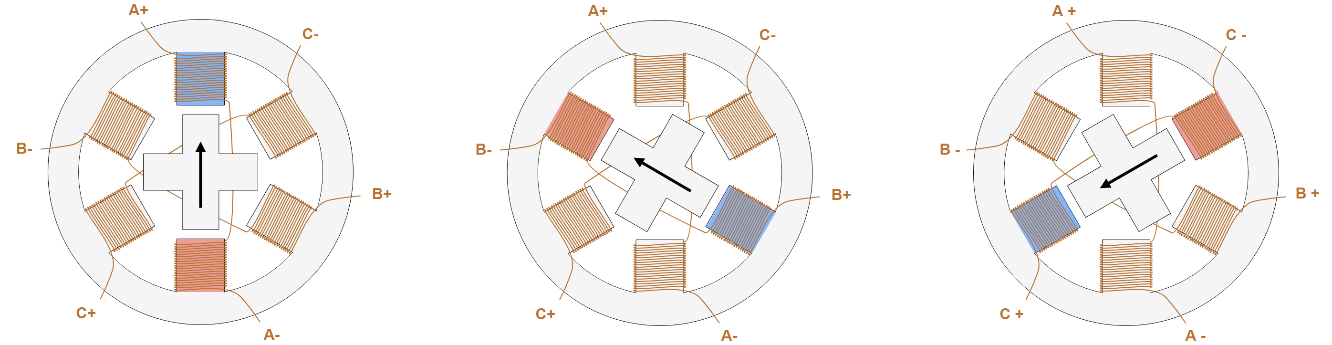
\includegraphics[\textwidth]{obrazky/stepper_principle}
    \caption{Working principle of a stepper motor~\cite{noauthor_stepper_nodate}.}
    \label{fig:stepper_working_principle}
\end{figure}

\subsubsection{Rotor}
There are three different constructions of rotors~\cite{noauthor_stepper_nodate}:
\begin{itemize}
    \item \textbf{Permanent magnet rotor} - utilizes a permanent magnet in the place of the stator.
    An advantage of this type of stator is good torque and also detent torque (the resistance of the motor shaft when no windings are energized)~\cite{noauthor_stepper_nodate}.
    \item \textbf{Variable reluctance rotor} - the rotor consists of a shaped iron core.
    The torques are generally lower and there is no detent torque~\cite{noauthor_stepper_nodate}.
    \item \textbf{Hybrid motor} - is created by combining a permanent magnet rotor with a variable reluctance rotor.
    There are two magnetic caps with teeths on top of each other that have an angular shift between them.
    The rotor is magnetized axially~\cite{noauthor_stepper_nodate}.
\end{itemize}

\subsubsection{Stator}
The construction of stator depends on the number of phases the motor has.
Every phase consists of two windings and the windings can be center-tapped or not, which determines if the motor is bipolar or unipolar.
With unipolar windings, the center tapped lead is connected to the input voltage and the direction of the magnetic field is controlled by connecting ground to the other leads.
Bipolar motors do not have center tapped lead and the coil itself is controlled using a H-bridge.

\subsection{Stepper motor driver IC comparison}
\label{subsec:stepper_ic}

\subsection{Trinamic motion control technologies}
\label{subsec:trinamic_tech}

